\documentclass[12pt]{article}
\usepackage[utf8]{inputenc} %decia latin1 
\usepackage{amsmath,amsfonts,amssymb,amsthm}
\usepackage[spanish, es-tabla]{babel}
\usepackage[auth-sc,affil-sl]{authblk}
\usepackage[latin1]{inputenc}
\usepackage[spanish]{babel}
\usepackage{graphicx}
\usepackage{natbib}
\usepackage{subfig}
%\usepackage[style=authoryear]{biblatex}
\usepackage[left=2cm,right=2cm,top=2cm,bottom=2cm]{geometry}
\usepackage{setspace}
\usepackage[all]{xy}
%\usepackage{fullpage}
\usepackage{longtable}
%\usepackage {fancyvrb}
\usepackage{fancyhdr}
%\usepackage{color}
\usepackage{pstricks}
\usepackage{amsthm}
%\usepackage{harvard}
\usepackage{float}
\usepackage{footmisc}
\usepackage{hyperref}
\usepackage{pdflscape}
\usepackage{textcomp}
\usepackage{xcolor}
\usepackage[table,xcdraw]{xcolor}
\usepackage{listings}


% Configuración para los bloques de código de R
\lstdefinestyle{Rstyle}{
    language=R,
    basicstyle=\small\ttfamily,
    backgroundcolor=\color{white},
    commentstyle=\color{green!50!black},
    keywordstyle=\color{blue},
    stringstyle=\color{red},
    showstringspaces=false,
    breaklines=true,
    frame=single,
    numbers=left,
    numberstyle=\tiny\color{gray},
    stepnumber=1,
    numbersep=5pt,
    tabsize=2,
    captionpos=b,
    belowcaptionskip=10pt,
    aboveskip=10pt
}

% Definición del entorno 'Rcode' para bloques de código de R
\lstnewenvironment{Rcode}[1][]{\lstset{style=Rstyle, #1}}{}


\usepackage[backend=bibtex, style=authoryear]{biblatex}
\addbibresource{biblio/biblio.bib}
%\usepackage[]{draftwatermark}
%\SetWatermarkText{24/05/21}
%\SetWatermarkLightness{0.8}
%\SetWatermarkScale{4}
\usepackage{subcaption}
\usepackage{tabularx}
\usepackage[colorinlistoftodos,prependcaption,textsize=tiny]{todonotes}%MONTXO
\newcommand{\duda}[1]{\todo[color=green!40]{#1}}
\newcommand{\sugerencia}[1]{\todo[color=orange!40]{#1}}
\newcommand{\corregir}[1]{\todo[color=red!40]{#1}}

\setlength{\parindent}{0.5cm}
\setlength{\textwidth}{6.3in}
\setlength{\topmargin}{-33pt}
\setlength{\oddsidemargin}{0pt}
\setlength{\evensidemargin}{0pt}
\setlength{\textheight}{8in}

% cosas del authblk
\setlength{\affilsep}{1mm}
\renewcommand\Authfont{\small} %\scshape\normalsize
\renewcommand\Affilfont{\itshape\small}

\renewcommand\Authsep{  }
\renewcommand\Authand{ }
\renewcommand\Authands{ }
\usepackage{multirow}

\begin{document}

\section{Aplicación Bayes Libro Baio}

En esta sección detallaremos la realización del análisis costo-efectividad presentado en el libro `Bayesian Cost-Effectiveness Analysis with the R package BCEA' (\cite{baio_bayesian_2017}) que presenta dos ejemplos, uno para la aplicación de una vacuna contra una enfermedad respiratoria y otro sobre un tratamiento para dejar de fumar.\
Se detallará el modelo económico y el modelo estadístico que está detras de la estimación de los parámetros, así como el proceso de Cadena de Markov para la estimación.\\

\subsection{Caso de la vacuna}

\subsubsection{Introducción}

Se supone que existe una enfermedad infecciosa que toda la población está en riesgo de contraer, un paciente que se agarra esta enfermedad (supón \textit{influenza}) puede tomar medicamentos de venta libre, o visitar su doctor, a veces la enfermedad es tratada con retro-virales, de persistir, en algunos casos pueden necesitar de una segunda visita al doctor, tratamientos anti-virales, internación ó incluso la muerte. Donde cada uno de estos escenarios numerados tienen un costo asociado.

Por otro lado, se tiene dos alternativas, disponer de una vacuna para todo aquel que desee vacunarse ($t=1$) contra no tener la vacuna disponible ($t=0$). Se desea poder analisar si la primera opción es costo-efectiva.\\

\subsubsection{Modelo}

En una población de tamaño $N$, la cantidad de individuos que se vacunan en el tratamiento $t=1$ (cuando la vacuna está disponible) viene dada por $V_1 \sim binomial(\phi,N)$, donde $\phi$ es la cobertura de la vacuna y claramente, en el tratamiento 0, $t=0$ se tiene $V_0=0$.\
Finalmente, se expresa $n_{tv}$ donde $v=0$ indica grupo de no vacunados y $v=1$ indica grupo de vacunados. Entonces queda definido $n_{t1}:= V_t$ y $n_{t0}:= N-V_t$.\
Luego, los resultados clínicos relevantes serán:
\begin{itemize}
\item $j=1$ \textit{infección de influenza} con probabilidad $\beta_1$.
\item $j=2$ \textit{visita de doctor} con probabilidad $\beta_2$.
\item $j=3$ \textit{complicaciones menores} con probabilidad $\beta_3$.
\item $j=4$ \textit{complicaciones mayores} con probabilidad $\beta_4$.
\item $j=5$ \textit{hospitalización} con probabilidad $\beta_5$.
\item $j=6$ \textit{muerte} con probabilidad $\beta_6$.
\item y $j=7$ \textit{eventos adversos a la vacunación} con probabilidad $\beta_7$.\\
\end{itemize}

Puntualmente para $\beta_1$ se tiene $\rho_v$ como la reducción proporcional de la tasa de infección para la población vacunada, es decir $\pi_{v}=\beta_1(1-\rho_v)$, para el grupo $v=0$ que son los individuos que no están vacunados tenemos una tasa de infección de $\beta_1$ ya que $\rho_0=0$.\\

Bajo las condiciones antes descritas, interesa ahora modelar la cantidad de pacientes pertenecientes a cada grupo. Empezando por la cantidad de infectados; la cantidad de infectados en cada uno de los grupos (vacunados y no vacunados) bajo cada uno de los tratamientos (vacunas disponibles y vacunas no disponibles) será:\\
\begin{itemize}

\item $I_{tv} \sim Binomial(\pi_v,n_tv)$.
\item luego para $j=2$ (\textit{visitas al médico}) en cada uno de los tratamientos disponibles, para cada grupo se tiene que $GP^{(1)}_tv \sim Binomial(\beta_2,I_{tv})$ ya que aquellos que se enferman de influenza son los que están en riesgo de visitar al doctor, y luego, todos los individuos que visitan al doctor son los que están en riesgo de tener uno de los resultados explicados anteriormente.
\item De esta manera, los individuos que presentan complicaciones menores $GP^{(2)}_{vt} \sim Binomial(\beta_3,GP^{(1)}_{tv})$,
\item los de complicaciones mayores $GP^{(3)}_{vt} \sim Binomial(\beta_4,GP^{(1)}_{tv})$,
\item los que tienen riesgo de hospitalización $H_{vt} \sim Binomial(\beta_5,GP^{(1)}_{tv})$ 
\item y los individuos que fallecen $D_{vt} \sim Binomial(\beta_6,GP^{(1)}_{tv})$.
\item Por último, los individuos con efectos adversos a la vacuna serán $EA_{tv} \sim Binomial (\beta_7,n_{tv})$ que será 0 en el escenario $t=0$ y también para el grupo de no vacunados ($v=o$) en el escenario $t=1$.
\end{itemize}

Por otra parte, el modelo incluye otros parámetros, que se detallan a continuación: un número de drogas antivirales ($\delta$) y la chance de recibir una prescripción médica para estos luego de la primera visita al doctor ($\gamma_1$), o al tener complicaciones menores ($\gamma_2$); la probabilidad de tomar medicamentos de venta libre ($\xi$); de tener una certificación laboral ($\eta$), por una cantidad de días ($\lambda$).\
Combinando estos parámetros con $N$ se tiene la cantidad esperada de individuos en cada uno de los eventos.\\

Para los costos se consideran los siguientes recursos: $h=1$ visita al doctor, $h=2$ episodio hospitalario, $h=3$ vacunación, $h=4$ tiempo para recibir la vacuna, $h=5$ días sin ir a trabajar, $h=6$ drogas antivirales, $h=7$ medicamentos de venta libre y $h=8$ viajes pare recibir la vacuna. Y cada recurso tiene un costo $\psi_h$ asociado.\\

Por último, se debe presentar la pérdida en la calidad de vida (\textit{QALY}), donde la pérdida de \textit{QALY} asociada a cada evento $j$ viene representada por $\omega_j$ y se asume que la visita al doctor no tiene pérdida de \textit{QALY} asociada, por lo que $\omega_2=\omega_3:=0$ y el resto de las $\omega_j 's$ son modeladas con una distribución log-normal.\\

Con la construcción de estos hiper-parámetros se puede construir \textbf{$\theta=(\theta^0,\theta^1)$} los parámetros poblacionales para cada uno de los dos escenarios, en donde se tiene que $\theta^0=(\beta_j,\gamma_1,\gamma_2,\delta,\xi,\eta,\lambda,\psi_h,\omega_j)$ y que $\theta^1=(\phi,\beta_j,\rho_v,\gamma_1,\gamma_2,\delta,\xi,\eta,\lambda,\psi_h,\omega_j)$ y sus distribuciones previas vienen dadas por la tabla \ref{tabla:99}. Donde el bloque 1 refiere a la proporción de vacunados; bloque 2 la probabilidad de ocurrencia de los distintos resultados, el 3 es el efecto de la vacuna sobre la probabilidad de infección, el 4 son otros parámetros, el 5 son los parámetros de costos, y el 6 son los parámetros que refieren a la pérdida de \textit{QALY} para cada uno de los eventos. La distribuciones son dadas por la literatura sobre el tema o por la opinión sobre experto, la función elegida responde directamente a la interpretación del parámetro. Para probabilidades o proporciones se eligió distribuciones \textit{Beta} que tienen recorrido en $\left[0,1\right]$, para cantidades enteras se eligió una distribución \textit{Poisson} que tiene recorridos en los naturales y para los costos se eligió una distribución \textit{Lognormal}, de forma tal que $Y=e^X \sim Lognormal$ si y solo si $X\sim Normal$. Se puede ver que los parámetros $\beta_5$ y $\beta_6$ que indican probabilidades tienen una distribución lognormal, pero los parámetros elegidos ($\mu$ y $\sigma$) que modelan la lognormal dan muy poca probabilidad a valores mayores a 1, para más detalles se puede ver \cite{baio_bayesian_2017}.

\begin{table}[]
\begin{tabular}{|l|l|l|l|l|l|l|}
\hline
Bloque             & Parametro  & Media    & 2,5\%    & Mediana  & 97,5\%   & Distribución              \\ \hline
1                  & $\phi$     & 0.435    & 0.245    & 0.436    & 0.625    & Beta(11.31,14.44)         \\ \hline
\multirow{7}{*}{2} & $\beta_1$  & 0.0701   & 0.0387   & 0.0680   & 0.1116   & Beta(13.01,172.38)        \\ \cline{2-7} 
                   & $\beta_2$  & 0.395    & 0.124    & 0.288    & 0.497    & Beta(5.80,13.80)          \\ \cline{2-7} 
                   & $\beta_3$  & 0.401    & 0.388    & 0.401    & 0.415    & Beta(1909.50,2851.86)     \\ \cline{2-7} 
                   & $\beta_4$  & 0.01339  & 0.00852  & 0.01322  & 0.01938  & Beta(20.94,1538.71)       \\ \cline{2-7} 
                   & $\beta_5$  & 0.000378 & 0.000223 & 0.000354 & 0.000616 & Lognormal(-7.91,14.93)    \\ \cline{2-7} 
                   & $\beta_6$  & 0.000748 & 0.000366 & 0.000702 & 0.001331 & Lognormal(-7.26,7.66)     \\ \cline{2-7} 
                   & $\beta_7$  & 0.1021   & 0.0255   & 0.0954   & 0.2265   & Beta(3.50,31.50)          \\ \hline
3                  & $\rho_1$   & 0.688    & 0.593    & 0.686    & 0.794    & Lognormal(-0.374,0.00524) \\ \hline
\multirow{6}{*}{4} & $\gamma_1$ & 0.420    & 0.417    & 0.420    & 0.423    & Beta(45471.58,62794.09)   \\ \cline{2-7} 
                   & $\gamma_2$ & 0.814    & 0.806    & 0.814    & 0.822    & Beta(7701.86,1759.89)     \\ \cline{2-7} 
                   & $\delta$   & 6.97     & 2        & 7        & 12       & Poisson(7)                \\ \cline{2-7} 
                   & $\xi$      & 0.950    & 0.940    & 0.950    & 0.959    & Beta(1804.05,94.95)       \\ \cline{2-7} 
                   & $\eta$     & 0.900    & 0.890    & 0.900    & 0.909    & Beta(3239.10,359.90)      \\ \cline{2-7} 
                   & $\lambda$  & 3.90     & 1.22     & 2.69     & 5.97     & Lognormal(0.98,0.17)      \\ \hline
\multirow{8}{*}{5} & $\psi_1$   & 20.55    & 12.36    & 19.77    & 32.07    & Lognormal(3.00,0.0606)    \\ \cline{2-7} 
                   & $\psi_2$   & 2661.92  & 1554.18  & 2575.67  & 4106.98  & Lognormal(7.85,0.0606)    \\ \cline{2-7} 
                   & $\psi_3$   & 7.21     & 4.22     & 6.95     & 11.42    & Lognormal(1.95,0.0606)    \\ \cline{2-7} 
                   & $\psi_4$   & 10.26    & 6.16     & 9.92     & 15.90    & Lognormal(2.29,0.0606)    \\ \cline{2-7} 
                   & $\psi_5$   & 46.31    & 27.2     & 44.96    & 70.69    & Lognormal(3.80,0.0606)    \\ \cline{2-7} 
                   & $\psi_6$   & 3.86     & 2.39     & 3.73     & 5.95     & Lognormal(1.31,0.0606)    \\ \cline{2-7} 
                   & $\psi_7$   & 1.592    & 0.949    & 1.562    & 2.452    & Lognormal(0.44,0.0606)    \\ \cline{2-7} 
                   & $\psi_8$   & 0.807    & 0.484    & 0.776    & 1.311    & Lognormal(-0.241,0.0606)  \\ \hline
\multirow{5}{*}{6} & $\omega_1$ & 4.26     & 2.14     & 4.05     & 7.59     & Lognormal(1.40,0.0933)    \\ \cline{2-7} 
                   & $\omega_4$ & 6.39     & 3.81     & 6.23     & 9.82     & Lognormal(1.82,0.606)     \\ \cline{2-7} 
                   & $\omega_5$ & 6.34     & 3.83     & 6.15     & 9.94     & Lognormal(1.82,0.0606)    \\ \cline{2-7} 
                   & $\omega_6$ & 15.20    & 9.09     & 14.88    & 23.34    & Lognormal(2.70,0.054)     \\ \cline{2-7} 
                   & $\omega_7$ & 0.556    & 0.316    & 0.541    & 0.932    & Lognormal(-0.634,0.0717)  \\ \hline
\end{tabular}
\caption{Tabla de distribuciones previas de los hiper-parámetros según información obtenida en la literatura y la opinión de expertos.
Fuente: 'Bayesian Cost-Effectiveness Analysis with the R package BCEA' capítulo:2}
\label{tabla:99}
\end{table}


En el repositorio de \textbf{osf} cuyo link se encuentra al inicio del documento, hay 4 `archivos.R' para poder hacer funcionar el modelo presentados por \cite{baio_bayesian_2017} en el libro \textit{`Bayesian Cost-Effectiveness Analysis with the R package BCEA'} y obtener estimaciones de la efectividad y los costos, así como un archivo llamado `vaccine.txt' con el modelo para hacer el método de Cadenas de Markov con MonteCarlo en un programa externo para esto como \textbf{JAGS} ó \textbf{BUGS}, ambos programas pueden ser ejecutados desde la consola de \textbf{R}.\
El archivo llamado \textit{`Utils.R'} contiene funciones útiles que se utilizan en los siguientes archivos, el archivo \textit{`LoadData.R'} contiene la obtención de los parámetros de las distribuciones previas según la tabla \ref{tabla:99}, y el archivo \textit{`RunMCMC.R'} tiene el código para poder correr las Cadenas de Markov con Métodos Montecarlo a través de JAGS ó BUGS. Por último, el archivo \textit{`ejemplo\_vacuna.R'} se tiene el código para representar los resultados del modelo bayesiano en términos de costo y efectividad para cada tratamiento según las fórmulas \ref{formula:costos} y \ref{formula:efectividad}, y luego se hace el análisis costo-efectividad correspondiente.\\


\begin{equation}
    c_{t}:= \frac{1}{N}\sum_{v=0}^1 \sum_{h=1}^8 N_{tvh}\psi_h
\label{formula:costos}
\end{equation}

Mientras tanto, si se llama $M_{tvj}$ a la cantidad de individuos en el tratamiento $t$, del grupo $v$ que experimentaron el episodio $j$, se puede calcular la efectividad media como:\\

\begin{equation}
    e_t := \frac{1}{N} \sum_{v=0}^1 \sum_{j=0}^7 M_{tvj}\omega_j
\label{formula:efectividad}
\end{equation}

Prestando atención a que esta pérdida de calidad está medida en días, se debe hacer la correspondiente transformación a \textit{QALY's} dividiendo entre 365. De esta manera se obtiene una efectividad y un costo promedio para cada una de las $n_{sims}$ simulaciones de la cadena.


\subsubsection{Los datos}

Para la obtención de los datos, se simula una población de tamaño $N=100000$, por ejemplo la cobertura de la vacuna está simulada y así también la cantidad de vacunados cuando la vacuna está disponible a partir de que en $t=1$ se tiene $V_t \sim Binomial(\phi,N)$. En lo que continúa de este capítulo se procede a hacer el análisis costo-efectividad manualmente en una primera instancia y luego con la \textit{librería `BCEA'}\duda{como citar el paquete} para los valores simulados de la población para cada iteración en el análisis bayesiano con los valores de los parámetros dados por \cite{baio_bayesian_2017} en `Bayesian Cost-Effectiveness Analysis with the R package BCEA' y luego se procederá a cambiar algunos valores de interés en los parámetros poblacionales y ver que cambios hay en el análisis costo-efectividad.\\

Para correr el modelo bayesiano se debe correr el archivo `RunMCMC.R' que al principio corre los archivos `Utils.R' que tiene funciones guardadas, y el archivo `LoadData.R' que carga algunos valores de los parámetros para las distribuciones previas.

\begin{Rcode}
# RunMCMC.R
# Cargar los paquetes OpenBUGS o JAGS from R 
# library(R2OpenBUGS)
library(R2jags)
library(tidyverse)
# Definir el directorio de trabajo
working.dir <- paste(getwd(),"/",sep="")
# Correr el archivo Utils.R con las funciones 
source("Utils.R")   #funciones utiles
# Cargar los datos en R simulados en LoadData
source("LoadData.R")  #simulacion de los datos poblacionales

# Definir la lista del nombre de las variables del modelo

data <- list(
"N","a.phi","b.phi","mu.rho","tau.rho","a.beta","b.beta","a.gamma","b.gamma","mu.omega","tau.omega","mu.psi","tau.psi","N.outcomes","N.resources","mu.lambda","tau.lambda","a.xi","b.xi","a.eta","b.eta","a.delta")  #nombre de las variables del modelo

# En el archivo vaccine.txt está el modelo escrito en formato JAGS
filein <- "vaccine.txt"   #modelo bayesiano

# definir los parametros
params <- c( "beta","phi","omega","rho","Infected","GP","Repeat.GP","Pneumonia","Hospital","Death","Mild.Compl","Trt","Adverse.events","n","gamma","delta","psi","lambda","pi","xi","eta")


# Generacion de los valores iniciales
inits <- function(){
  list(
phi = runif(1), beta = runif(N.outcomes,0,1), rho = c(NA,runif(1)), gamma = runif(2,0,1), delta = rpois(1,2), omega = c(runif(1), NA, NA, runif(1), NA, runif(2,0,1)), psi = runif(N.resources,0,10), lambda = runif(1), eta = runif(1), xi = runif(1))
}

# Definir el numero de iteraciones, la cantidad de calentamiento y la cantidad que se tomara efectivamente para eliminar la autocorrelacion
n.iter <- 100000
n.burnin <- 9500
n.thin <- floor((n.iter-n.burnin)/500)

# 1. Para correr en OpenBUGS
# vaccine <- bugs(data, inits, params, model.file=filein,n.chains=2, n.iter, n.burnin, n.thin, DIC=FALSE, working.directory=working.dir, debug = T)

# 2. Para correr en JAGS
vaccine <- jags(data, inits, params, model.file=filein,n.chains=2, n.iter, n.burnin, n.thin,
                DIC=FALSE, working.directory=working.dir, progress.bar="text")

# Imprimir el restulado
print(vaccine, digits=3,intervals=c(0.025, 0.975))


# In OpenBUGS:
# attach.bugs(vaccine)
# vinculamos los objetos del modelo bayesiano en JAGS:
attach.jags(vaccine)

#traceplot(vaccine) #para ver la convergencia de las cadenas

\end{Rcode}


En el archivo llamado `ejemplo\_vacuna.R' se encuentra inicialmente los códigos necesarios para transformar los datos obtenidos en cada paso de la simulación en un valor de la efectividad y del costo (guardados en las matrices \textit{e} y \textit{c} respectivamente).\
Además, en caso de no poder haber corrido el modelo en `JAGS' ó `BUGS', o haber tenido algun inconveniente se brinda un archivo llamado `Vaccine.RData' (que se puede cargar al inicio del archivo \textit{`ejemplo\_vacuna}) brindado por Baio en (\url{"https://gianluca.statistica.it/books/bcea/code/vaccine.RData"}) que tiene los valores de todos los parámetros en cada una de las simulaciones de la cadena de Markov para poder repetir el mismo análisis que se hace a continuación (\footnote{los valores presentados en el documento son los obtenidos al cargar el archivo `Vaccine.RData', en caso de transformar los datos obtenidos en `RunMCMC.R' en efectividad y costo puede llevar a pequeñas diferencias respecto a los valores plasmados en el documento}). Al inicio del código se procesa y se obtiene el valor de la efectividad para cada uno de los tratamientos en cada una de las 1000 simulaciones, y análogamente para los costos.\
Posteriormente se haya las diferencias de medias en las efectividades y los costos de cada tratamiento para obtener la estimación de $\widehat{ICER_{1,0}}$ en cada simulación.\

\begin{Rcode}
# ejemplo_vacuna.R

# creacion de los valores de efectividad
QALYs.inf <- QALYs.pne <- QALYs.hosp <- QALYs.adv <- 
QALYs.death <- matrix(0,n.sims ,2)

# los valores de los parametros son obtenidos en la cadena de markov
for (t in 1:2) {
  QALYs.inf[,t] <- ((Infected[,t,1] + Infected[,t,2])*omega[,1]/365)/N
  QALYs.pne[,t] <- ((Pneumonia[,t,1] + Pneumonia[,t ,2])*omega[,4]/365)/N
  QALYs.hosp[,t] <- ((Hospital[,t,1] + Hospital[,t,2])*omega[,5]/365)/N
  QALYs.death[,t] <- ((Death[,t,1] + Death[,t,2])*omega[ ,6])/N
}
QALYs.adv[,2] <- ( Adverse.events* omega[,7]/365)/N
e <- -(QALYs.inf + QALYs.pne + QALYs.adv + QALYs.hosp + QALYs.death)


# creacion de los valores de costos
cost.GP <- cost.hosp <- cost.vac <- cost.time.vac <- cost.time.off <- cost.trt1 <- cost.trt2 <- cost.otc <- cost.travel <- matrix(0,n.sims ,2)
for (t in 1:2) {
  cost.GP[,t] <- (GP[,t,1]+GP[,t,2]+ Repeat.GP[,t,1]+
  Repeat.GP[,t,2])*psi[,1]/N
  cost.hosp[,t] <- (Hospital[,t ,1]+ Hospital[,t ,2])*psi[ ,2]/N
  cost.vac[,t] <- n[,2,t]*psi[,3]/N
  cost.time.vac[,t] <- n[,2,t]*psi[,4]/N
  cost.time.off[,t] <- (Infected[,t ,1]+ 
  Infected[,t ,2])*psi[ ,5]*eta* lambda/N
  cost.trt1[,t] <- (GP[,t,1]+GP[,t,2])*gamma[ ,1]*psi[,6]* delta/N
  cost.trt2[,t] <- (Repeat.GP[,t,1]+ 
  Repeat.GP[,t,2])*gamma[ ,2]*psi[,6]* delta/N
  cost.otc[,t] <- (Infected[,t ,1]+ Infected[,t ,2])*psi[ ,7]*xi/N
  cost.travel[,t] <- n[,2,t]*psi[ ,8]/N
}

c <- cost.GP + cost.hosp + cost.vac + cost.time.vac + 
cost.time.off + cost.trt1 + cost.trt2 + cost.travel + cost.otc
\end{Rcode}

Luego de construidos los valores de costo y efectividad para cada paso de la simulación procedemos a estimar el valor del $ICER_{1,0}$ y construir el plano costo-efectividad con cada una de nuestra simulaciones.

\begin{Rcode}
evaluacion <- cbind(e,c)  #se juntan todos los resultados obtenidos
evaluacion <- as.data.frame(evaluacion)
colnames(evaluacion) <- c("efectividad_t0","efectividad_t1","costos_t0","costos_t1")


# se calcula las diferencias de efectividad y costo en cada simulacion y se calcula el ICER para cada simulacion
evaluacion <- evaluacion %>% mutate(
  dif_efect = efectividad_t1 - efectividad_t0,
  dif_cost = costos_t1 - costos_t0,
  ICER_10 = dif_cost/dif_efect
)

prom_ICERS=mean(evaluacion$ICER_10)  #esta NO es la estimacion puntual del ICER


#esta si es:
resumen <- evaluacion %>% summarise(
  prom_c1 = mean(costos_t1),
  prom_c0 = mean(costos_t0),
  prom_e1 = mean(efectividad_t1),
  prom_e0 = mean(efectividad_t0)
)

est_ICER <- resumen %>% 
  summarise(ICER = (prom_c1 - prom_c0)/(prom_e1 - prom_e0))

\end{Rcode}

\begin{table}[ht]
\centering
\begin{tabular}{rrr}
  \hline
 & Tratamiento 0 & Tratamiento 1 \\ 
  \hline
Efectividad & -0.0011 & -0.0008 \\ 
  Costos & 9.8145 & 14.8643 \\ 
   \hline
\end{tabular}
\caption{Costo y efectividad promedio de las simulaciones}
\label{tab:resumen_medias}
\end{table}


De esta manera se obtiene un $\widehat{ICER_{1,0}}=\frac{\bar{c_1}-\bar{c_0}}{\bar{e_1}-\bar{e_0}}=\frac{14.8643-9.8145}{-0.0008-(-0.0011)}=20302.9$.\
Debe observarse que no es el mismo resultado que calcular el $ICER_{1,0}$ en cada paso de la simulación, y luego calcular el promedio, estimarlo de esa manera sería un error. Lo que si es útil para el análisis es graficar en el plano costo-efectividad cada pareja de diferencia de efictividad y diferencia de costo obtenida en cada simulación, y calcular la proporción de estas que se encuentran por debajo de nuestra frontera de aceptación. Obteniendo un gráfico como el siguiente:

\begin{figure}[H]
    \centering
    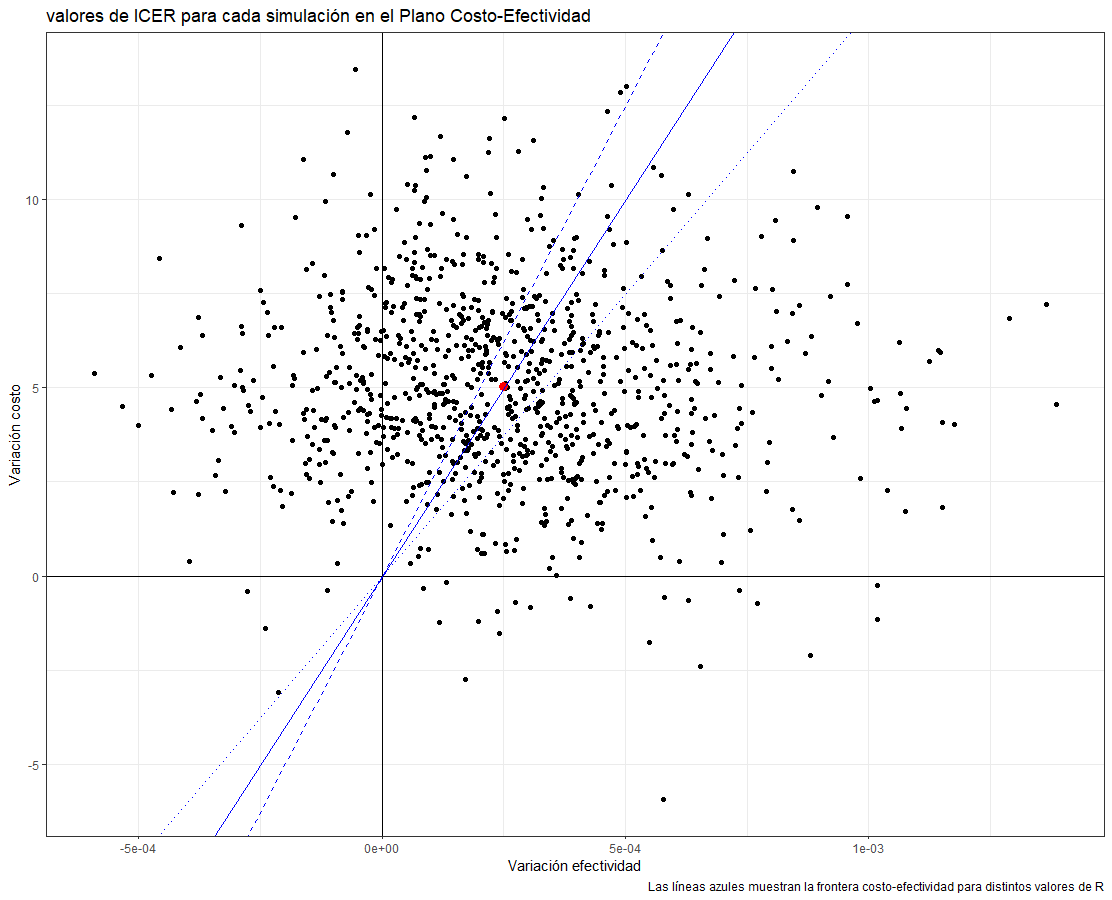
\includegraphics[width=0.81\textwidth]{grafi/plano_icer_simulaciones.jpg}
    \caption{Plano Costo-efectividad de ICER's en cada simulación y distintas fronteras costo-efectivas.}
    \label{fig:61}
\end{figure}

Por otro lado, este análisis se puede hacer utilizando la librería \textit{`BCEA'} que cuenta con una función que recibe (idealmente) las simulaciones obtenidas en cada paso de la cadena de markov para la efectividad promedio y para el costo promedio de la población en cada tratamiento, pero adicionalmente puede recibir los resultados obtenidos a partir de varias simulaciones obtenidas con bootstrap.\
La función que se utiliza se llama \texttt{bcea} y recibe dos matrices, una para la efectividad en la que cada fila es el resultado obtenido en cada paso de la simulación y cada columna es un tratamiento (la matriz obtenida anteriormente en las primeras lineas del archivo `ejemplo\_vacuna.R'), y otra matriz análoga para los costos. Luego se debe fijar cuál es el tratamiento que usaremos de referencia, como $t=1$ en la fórmula del ICER, ya que la función puede recibir matrices de más de dos columnas, es decir, más de dos tratamientos, y por defecto comparará la primer columna contra el resto. En este caso, como la efectividad y los costos del tratamiento alternativo están en la columna 2, se pone \texttt{ref=2}, luego adicionalmente se le puede pasar el nombre de los tratamientos en un vector, de lo contrario le pondrá 'Intervention 1', 'Intervention 2'... por último, se le puede agregar un vector de valores de \textit{R} (disposición máxima a pagar) en el argumento \texttt{k} para que calcule la probabilidad de aceptar el tratamiento alternativo para esos valores, de lo contrario se le puede dar un valor máximo de R en el argumento \textit{Kmax} que indica hasta que valor deseamos observar los resultados en los gráficos que se generan automáticamente. En caso de darle un valor de \textit{Kmax}, la probabilidad de aceptar el nuevo tratamiento se calculará para una grilla de 501 valores entre 0 y \textit{Kmax}.\

\begin{Rcode}
    # analisis con la libreria bcea

library(BCEA)

tratamientos <- c("status_quo", "vacunacion")  #etiqueta a cada tratamiento

analisis <- bcea(e,c,ref=2,intervention = tratamientos, Kmax=50000) 

plot(analisis)  # graficos de bcea

summary(analisis)  # resumen
\end{Rcode}

Se puede ver que si uno corre \texttt{class(analisis)} en la consola, este objeto es una lista del tipo `bcea', que es justamente la clase de objeto que genera la función \texttt{bcea}, luego al aplicarle la función \texttt{plot} de \texttt{R} esta generará gráficos especiales para este tipo de objeto. Ya que esta función básica del R genera gráficos especiales para algunos tipos de objetos determinados, como pueden ser modelos lineales, o series de tiempo.


\begin{figure}[H]
    \centering
    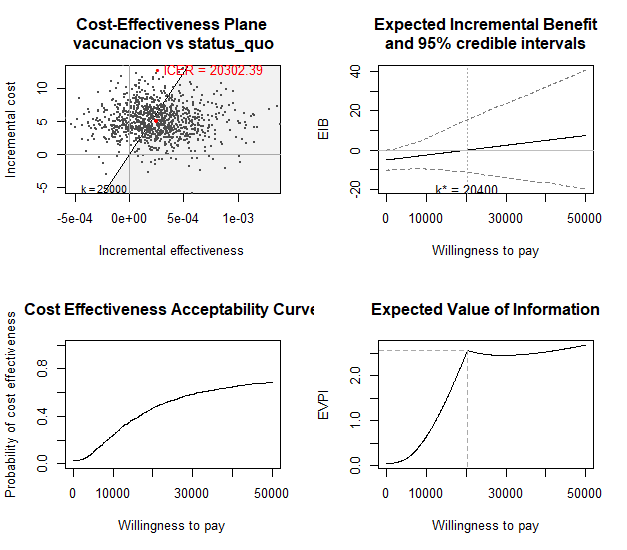
\includegraphics[width=1\textwidth]{grafi/plot_bcea.jpg}
    \caption{Gráfico de objeto BCEA}
    \label{fig:62}
\end{figure}


En el gráfico de arriba a la izquierda de la figura \ref{fig:62}, se tiene un gráfico parecido al hecho anteriormente, en donde tenemos todos los puntos de las variaciones de efectividad y de costo, con el promedio resaltado y una recta con pendiente igual a la disposición a pagar por unidad extra de efectividad. En el gráfico de arriba a la derecha se tiene el Beneficio Neto esperado y un intervalo de confianza al 95\% para distintos valores de la disposición a pagar. En el gráfico de abajo a la izquierda se tiene la probabilidad de aceptar el nuevo tratamiento para distintos valores de la disposición a pagar, y en el gráfico de abajo a la derecha tenemos el valor esperado de la información para distintos valores de la disposición a pagar.\\

Adicionalmente, se puede utilizar la función \textit{summary} disponible en \textbf{R}, que devuelve un resúmen, en este caso, de un objeto de clase `bcea'. Esta función devuelve un resumen indicando cual es el tratamiento de referencia y cual el de comparación, los valores de `R' para los cuáles elegir cada tratamiento, y para un $R=25000$ (por defecto, que se puede cambiar con el argumento \textit{wtp}), el beneficio neto esperado en cada tratamiento, y luego el incremento del beneficio neto, la probabilidad de que el nuevo tratamiento sea costo-efectivo y el ICER calculado.\\

Para facilitar la observación de los datos se cuenta con una función para ver detalladamente cada gráfico que iremos viendo a continuación. Opcionalmente se le puede agregar el comando \texttt{graph = "ggplot2"} para que el gráfico sea del estilo de la librería ``ggplot2''.\

\begin{Rcode}
ceplane.plot(analisis, graph=``ggplot2'')  #plano costo-efectividad
contour(analisis)  #plano con regiones
contour2(analisis)
\end{Rcode}

También se presenta el gráfico obtenido con la función \texttt{contour} (figura \ref{fig:64}), que divide al plano costo-efectividad en 5 regiones, teniendo al 20\% de la distribución conjunta en cada una de ellas. Además indica la probabilidad de caer en cada uno de los cuadrantes del plano costo-efectividad, por otro lado la función \texttt{contour2} produce el mismo gráfico que \texttt{ceplane.plot} pero con los contornos.


\begin{figure}[H]
    \centering
    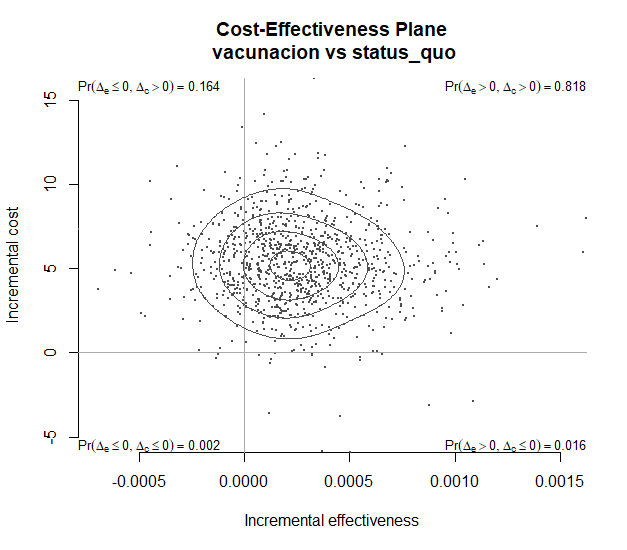
\includegraphics[width=.65 \textwidth]{grafi/countor_plot.jpg}
    \caption{Gráfico obtenido con la función contour del paquete ``BCEA''}
    \label{fig:64}
\end{figure}

\subsubsection{Análisis de Sensibilidad Probabilística}

El análisis de sensibilidad probabilística (Probabilistic Sensitivity Analysis (PSA)) es una técnica para estudiar la incertidumbre sobre los parámetros de los modelos, y es ampliamente utilizada en la evaluación económica en salud, nosotros lo usaremos para la diferencia en efectividad y costo y el paquete \texttt{bcea} a través de los gráficos `básicos' hace esta tipo de análisis.\

Además, usando la función \texttt{sim\_table} sobre el objeto de clase \textbf{bcea} podemos acceder a los valores de la utilidad de cada tratamiento y otras cosas que se explicaran más adelante para  cada paso de la simulación, dado un valor de disponibilidad a pagar.


\begin{Rcode}
tabla_psa <- sim_table(analisis,wtp=25000)
head(tabla_psa$Table)
\end{Rcode}

\begin{table}[ht]
\centering
\begin{tabular}{lrrrrrr}
  \hline
simulación & U1 & U2 & U* & IB2\_1 & OL & VI \\ 
  \hline
1 & -42.02 & -38.53 & -38.53 & 3.49 & 0.00 & -3.24 \\ 
  2 & -25.70 & -32.64 & -25.70 & -6.94 & 6.94 & 9.58 \\ 
  3 & -40.00 & -34.69 & -34.69 & 5.31 & 0.00 & 0.60 \\ 
  4 & -58.70 & -36.28 & -36.28 & 22.42 & 0.00 & -0.99 \\ 
  5 & -34.88 & -29.62 & -29.62 & 5.26 & 0.00 & 5.67 \\ 
  6 & -45.63 & -45.98 & -45.63 & -0.35 & 0.35 & -10.35 \\ 
   \hline
\end{tabular}
\caption{Salida de \texttt{head(tabla\_psa\$Table)}}
\label{Tabla:Resultadosevpi}
\end{table}


Una tabla como la presentada en (\ref{Tabla:Resultadosevpi}) es calculada para cada valor de la disponibilidad a pagar \footnote{cada uno de los valores de la grilla de largo 501 que va de 0 a \texttt{Kmax}}, en esta se encuentra la utilidad del tratamiento de referencia para este valor de disponibilidad a pagar ($U1$), la utilidad del tratamiento nuevo ($U2$), la mejor utilidad para esa simulación ($U^*$), el beneficio incremental al cambiar de tratamiento ($IB2\_1$), el costo de oportunidad ($OL$) y el valor de la información $VI$.

Se puede observar que $U^* = max(U1,U2)$ y será igual a la utilidad obtenida si se elige el mejor tratamiento en esa simulación.
Luego, el costo de oportunidad para cada simulación será:

\begin{equation}
        OL(\theta) = U^{*}(\theta)-U(\theta^\tau)
\end{equation}

Donde $U(\theta^\tau)$ es la utilidad obtenida en esta simulación cuando se elige el tratamiento más costo-efectivo para todas las simulaciones al valor de la disponibilidad a pagar seleccionado. Recordando que se tuvo:

$$
\widehat{ICER_{1,0}} = 20302,9
$$

Para la tabla calculada con una disponibilidad a pagar de $\$25000$ se espera que muchos valores de $OL$ sean $0$, ya que en muchos casos, el mejor tratamiento para esa simulación será el mismo que el elegido tomando en cuentas todas las simulaciones. Por último, el valor esperado de la información para un valor de disponibilidad a pagar será:

\begin{equation}
\begin{split}
EVPI =  & \mathbb{E}(OL(\theta)) \\
\widehat{EVPI} = & \overline{OL(\theta)} = \frac{\sum_{i \in sims} OL_i (\theta)}{n.sims}
\end{split}
\label{eq:evpi}
\end{equation}

Se puede ver que cambiando el valor de la disponibilidad a pagar y calculando esta tabla, al imprimir las primeras simulaciones se obtendrá que cambia la utilidad de cada tratamiento y el mejor tratamiento para dicho nivel, así cómo los valores de la pérdida de oportunidad para cada simulación. Por ejemplo, para la disponibilidad a pagar de $\$40000$ se tendrá que más simulaciones resultan costo-efectivas cuando se elige el segundo tratamiento, y no tendrán pérdida de oportunidad. Mientras que cuando se calcula con una disponibilidad a pagar menor se tendrá que el primer tratamiento será el elegido cuando se tiene en cuenta todas las simulaciones, y habrá pérdida de oportunidad en aquellas en que el segundo tratamiento es más efectivo.

\begin{table}[ht]
\centering
\begin{tabular}{rrrrrrr}
  \hline
 & U1 & U2 & U* & IB2\_1 & OL & VI \\ 
  \hline
1 & -52.18 & -46.71 & -46.71 & 5.47 & 0.00 & 0.84 \\ 
  2 & -33.21 & -42.52 & -33.21 & -9.31 & 9.31 & 14.33 \\ 
  3 & -54.97 & -43.73 & -43.73 & 11.23 & 0.00 & 3.81 \\ 
  4 & -87.82 & -48.52 & -48.52 & 39.29 & 0.00 & -0.98 \\ 
  5 & -51.09 & -36.83 & -36.83 & 14.26 & 0.00 & 10.71 \\ 
  6 & -66.57 & -65.07 & -65.07 & 1.49 & 0.00 & -17.53 \\ 
   \hline
\end{tabular}
\caption{Salida de \texttt{head(tabla\_psa\$Table)} para una disponibilidad a pagar de $\$40000$}
\end{table}

\begin{table}[ht]
\centering
\begin{tabular}{rrrrrrr}
  \hline
 & U1 & U2 & U* & IB2\_1 & OL & VI \\ 
  \hline
1 & -31.86 & -30.36 & -30.36 & 1.50 & 1.50 & -9.88 \\ 
  2 & -18.20 & -22.77 & -18.20 & -4.57 & 0.00 & 2.27 \\ 
  3 & -25.03 & -25.64 & -25.03 & -0.62 & 0.00 & -4.56 \\ 
  4 & -29.58 & -24.04 & -24.04 & 5.55 & 5.55 & -3.56 \\ 
  5 & -18.67 & -22.41 & -18.67 & -3.73 & 0.00 & 1.80 \\ 
  6 & -24.70 & -26.90 & -24.70 & -2.20 & 0.00 & -4.23 \\ 
   \hline
\end{tabular}
\caption{Salida de \texttt{head(tabla\_psa\$Table)} para una disponibilidad a pagar de $\$10000$}
\end{table}

Luego, para poder graficar el valor esperado de la información se calcula con la fórmula \ref{eq:evpi} para cada valor de la disponibilidad a pagar (en este caso una grilla) y se obtiene el gráfico, dónde se puede ver que en el valor de $\widehat{ICER_{1,0}}$ se tiene un máximo.

\begin{Rcode}
# graficos PSA

evi.plot(analisis, graph = "ggplot2")  #valor esperado de la informacion
ib.plot(analisis, graph = "ggplot2", k=25000)  #densidad incremento del beneficio
ceac.plot(analisis, graph = "ggplot2")  #curva de aceptacion
\end{Rcode}


\begin{figure}[H]
    \centering
    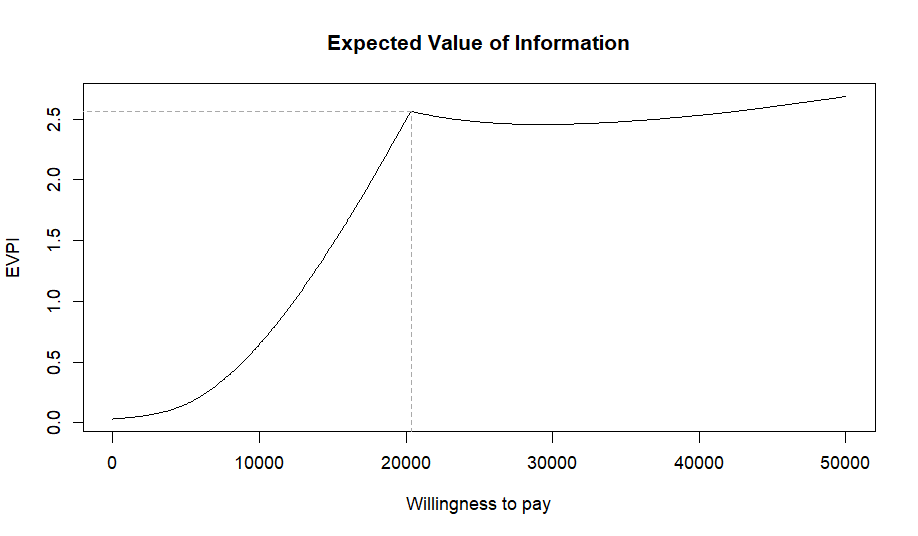
\includegraphics[width=1 \textwidth]{grafi/evi_plot.jpg}
    \caption{Gráfico del valor esperado de la información perfecta}
    \label{fig:65}
\end{figure}

El \textbf{EVPI}, que está medido per-capita puede verse como el beneficio esperado por conocer los verdaderos valores de los parámetros, es el valor máximo per-capita que se está dispuesto a pagar para conocer los verdaderos valores de los parámetros del modelo.\\

Otros gráficos que forman parte del análisis de sensibilidad probabilístico son la densidad del Incremento del Beneficio para un valor de disponibilidad a pagar (fifura \ref{fig:63}) que se calcula con métodos no paramétricos con los valores de $IB1\_2$ de la tabla para una disponibilidad a pagar dada.

\begin{figure}[H]
    \centering
    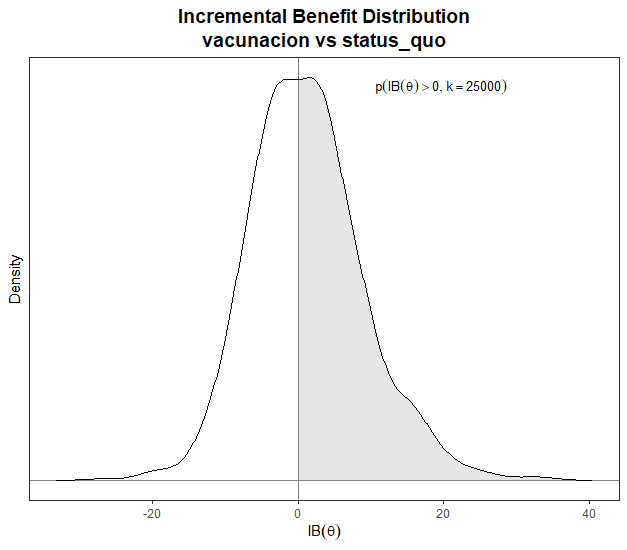
\includegraphics[width=.65\textwidth]{grafi/ib_plot.jpg}
    \caption{Densidad del incremento de beneficio neto estimado con un Núcleo Gaussiano para un R=25.000}
    \label{fig:63}
\end{figure}

También la curva de aceptación costo-efectividad se calcula a partir de esta tabla, y para cada valor de la disponibilidad a pagar calcula la proporción de simulaciones para las cuáles el tratamiento alternativo es costo-efectivo.

\begin{figure}[H]
    \centering
    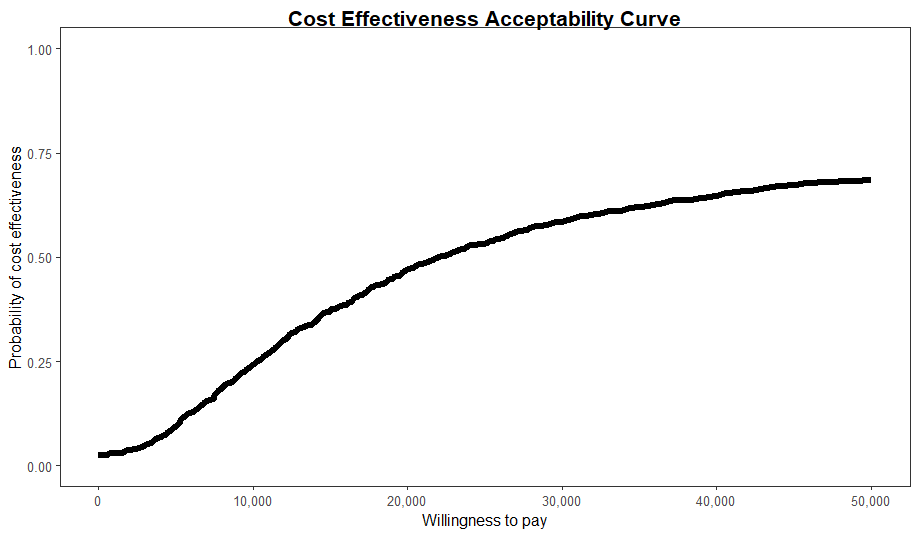
\includegraphics[width=.65\textwidth]{grafi/ceac_plot.jpg}
    \caption{Curva de Aceptación Costo-Efectividad}
    \label{fig:70}
\end{figure}



\subsubsection{Cambiando Algunos Parámetros}

Como se comentó anteriormente nos será de interés cambiar el valor de algunos parámetros de la población y su información previa y observar cómo cambia la estimación del ICER y la probabilidad de aceptar el nuevo tratamiento para distintos valores de la disponibilidad a pagar.

\begin{center}
    \textbf{Cobertura de la vacuna}
\end{center}

En el archivo `RunMCMC.R' se puede ver que el valor inicial para el parámetro $\phi$ es simulado con una variable aleatoria uniforme entre 0 y 1, y la información previa se distribuye $Beta(\alpha,\beta)$ donde los valores de $\alpha$ y $\beta$ se calculan a partir del código `Utils.R' y `LoadData.R'.

Se comenzará cambiando los valores iniciales en el objeto \texttt{inits} que simula los valores poblacionales, inicialmente se tiene que la cobertura de la vacuna se simula con una distribución $Uniforme(0,1)$. Probaremos cambiando por una $Uniforme(0.8,1)$ para tener mayor cobertura en la población simulada.

\begin{Rcode}
inits2 <- function(){
  list(
phi = runif(1, min=0.8, max=1), beta = runif(N.outcomes, 0, 1), rho = c(NA, runif(1)), gamma = runif(2, 0, 1), delta = rpois(1, 2), omega = c(runif(1), NA, NA, runif(1), NA, runif(2,0,1)), psi = runif(N.resources,0,10), lambda = runif(1), eta=runif(1), xi = runif(1))
}

\end{Rcode}

Se continua corriendo el resto del código, y cuando se corre el modelo en \textbf{JAGS} se cambia lo que antes era \texttt{inits} por \texttt{inits2}.

\begin{Rcode}
vaccine2 <- jags(data, inits2, params, model.file = filein, n.chains=2, n.iter, n.burnin, n.thin, DIC=FALSE, working.directory = working.dir, progress.bar = "text")
\end{Rcode}

Se continua transformando los datos en las simulaciones en términos de costo y efectividad con el código de `ejemplo\_vacuna.R' que fue presentado anteriormente y se le aplica la función \texttt{bcea} y calculamos el $\widehat{ICER_{0,1}}$.\

Luego vamos a hacer lo mismo pero en el otro sentido, bajando la cobertura de la vacuna en los datos simulados por una distribución $Uniforme(0,0.2)$, y se vuelve a estimar $\widehat{ICER_{0,1}}$.

En este caso utilizaremos el archivo `cambio\_parametros.R', al inicio se corre las mismas líneas que en `RunMCMC.R' y se simulan los datos originales obteniendo una estimación del ICER de $19339.4$, que es diferente al presentado anteriormente que estaba calculado con los datos brindados, y ya se comentó esta posible diferencia. Esto se hace para luego poder compararlo con los ICER's cuando se cambian los parámetros de los datos, ya que el ICER de los datos brindados no es comparable. 


\begin{table}[ht]
\centering
\begin{tabular}{ll}
  \hline
Simulación de los datos & $\widehat{ICER_{1,0}}$ \\ 
  \hline
Original & 19339.44 \\ 
$\phi \sim U(0.8 ; 1)$ & 19281.51 \\ 
$\phi \sim U(0 ;0.2)$ & 20509.63 \\ 
   \hline
\end{tabular}
\caption{Estimación del ICER para distintos valores de la cobertura de la vacuna}
\label{tabla:cambio_cobertura}
\end{table}


En la tabla \ref{tabla:cambio_cobertura} se puede ver que aumentando la cobertura de los datos disminuye el ICER, es decir, ahora por cada punto de efectividad extra el costo es menor al caso original, mientras que cuando disminuye la cobertura de los datos aumenta el ICER.

Si vemos el plano costo-efectividad de los 3 casos veremos que el promedio de la diferencia de la efectividad y el costo queda en el \textbf{cuadrante 1} por lo que tiene sentido comparar los valores de los ICER's que son todos positivos.

\begin{center}
    \textbf{Disminución en la probabilidad de contagio con vacuna}
\end{center}

Ahora probaremos cambios en $\rho$ que es un parámetro que cambia la probabilidad de contagio ($\pi$) para los individuos que se vacunan a través de la fórmula:

\begin{equation}
    \pi_v = \beta_1 (1-\rho)
\end{equation}

Donde $\beta_1$ es la probabilidad de contagio para los individuos que no se vacunan. Por lo que a mayor valor de $\rho$ disminuirá la probabilidad de contagio de los individuos que se vacunan, y a menor valor, tendrá menos influencia la vacuna.\\

Para asignar una disminución del $\%90$ en la probabilidad de contagio para el grupo de vacunados se cambió el valor del parámetro \texttt{rho} en la lista de valores iniciales, y lo mismo se hizo para asignar una disminución del $\%10$ en la probabilidad de contagio.

\begin{Rcode}
    
inits4 <- function(){
list(
phi = runif(1), beta = runif(N.outcomes, 0, 1), rho = c(NA, 0.9), gamma = runif(2, 0, 1), delta = rpois(1, 2), omega = c(runif(1), NA, NA, runif(1), NA, runif(2,0,1)), psi = runif(N.resources,0,10), lambda = runif(1), eta=runif(1), xi = runif(1))
}

\end{Rcode}

Luego, los resultados obtenidos para cada escenario son: 

\begin{table}[ht]
\centering
\begin{tabular}{ll}
  \hline
 Valores de los datos & $\widehat{ICER_{1,0}}$ \\ 
  \hline
 Original & 19339.44 \\ 
 rho=0.9 & 19301.71 \\ 
 rho=0.5 & 20849.52 \\ 
 rho=0.1 & 20891.45 \\ 
   \hline
\end{tabular}
\caption{Estimación del ICER para distintos valores de la disminución de la probabilidad de contagio con vacuna}
\label{tabla:cambio_influencia}
\end{table}

En la tabla \ref{tabla:cambio_influencia} se puede ver que cuando el valor de $\rho$ aumenta, es decir disminuye la probabilidad de contagio, el ICER disminuye, porque se está mejorando la efectividad de un tratamiento al otro, obteniendo un costo menor por cada punto extra de efectividad. Mientras que cuando la incidencia de la vacuna en la probabilidad de contagio no es tan grande, $\rho=0.5$ ó $\rho=0.1$ aumenta el ICER, es menos costo-efectivo tener la vacuna disponible para toda la población.







\end{document}
